\section{Propositional Logics}\label{cha:FormulaTensors}

Propositional logics describes systems with $\atomorder$ binary categorical variables, which are called atoms and denoted by $\atomicformulaof{\atomenumerator}$ for $\atomenumeratorin$.
Indices $\atomlegindexof{\atomenumerator}\in[2]$ to the atoms $\atomenumeratorin$ enumerate the $2^\atomorder$ states of these systems, which are called worlds.
In each world indexed by $\atomindices$ the indices $\atomicformulaof{\atomenumerator}$ encode whether the corresponding variable is $\truesymbol$. 

% Structure
We here choose a semantic centric approach to propositional logic, by defining formulas as binary tensors.
Then we investigate the corresponding syntax of formulas as specification of a tensor network decomposition of the relational encoding of formulas.


\subsection{Encoding of Booleans}

Propositional logic amounts to reason about Boolean variables, which are categorical variables with $2$ possible values.
Before applying this insight in the representation of propositional formulas, we first investigate how Boolean calculus can be represented by multilinear operations.

\subsubsection{Booleans as categorical variables}


%\begin{remark}[Boolean Calculus to Binary Calculus] % This is Coordinate Calculus, Happening on the Coordinates during Binary Tensor Contractions
	%We use an embedding of truth assignments to $\{0,1\}=[2]$ and store in large vectors, restructured as tensors, truths to sets of formulas.
	To represent Booleans by categorical variables $\catvariable$ with two states we use the following standard group homomorphism % (this is standard, also build in python)
		\[ \big(\{\truesymbol,\falsesymbol\},\land\big) \quad \text{and} \quad \big(\{ 1,0\},\cdot\big) \]
	by the map
    		\[ [\cdot]:\{\truesymbol,\falsesymbol\} \rightarrow \{1,0\} \]
	defined as
	    	\[ [\truesymbol] = 1 \quad , \quad [\falsesymbol] = 0 \, . \]
	The multiplication is performed in the binary tensor contractions and can thus be interpreted as the $\land$ connective performed on Boolean coordinates.
%\end{remark}


% Expressivity Issues
While the conjunction of is in this embedding performed by multiplications, operations like the negation
	\[ [\lnot X] = 1 - [X]  \]
are affine linear.
Direct applications of these affine linear operations to perform logical calculus will be discussed later in Section~\ref{sec:effectiveGroundingCalculus}.

However, in this chapter we will circumvent the problems arising with affine linearity by using the one-hot encoding of Booleans.


\subsubsection{One-hot Encoding} % This is what Basis Calculus does! Refer to that here?

Booleans are categorical variables with $\catdim=2$ states, where we interpret the states $[2]=\{0,1\}$ by $\{\truesymbol,\falsesymbol\}$.
The one-hot encoding of Booleans
	\[ \onehotmap: [2] \rightarrow \{\fbasis[\catvariable] ,\tbasis[\catvariable] \}  \subset \rr^2 \]
is thus understood as an encoding of truth values.

%% Expressivity
As discussed before, the one-hot encoding is rich enough to represent any function of the state by a linear function on the encoding.
The truth of formulas is a function of the truth of atomic formulas, and thus representable by linear functions of the one-hot encodings.




\subsection{Semantics of Propositional Formulas}

The epistemological commitments are whether the state is $\truesymbol$ or $\falsesymbol$ reflected by the coordinate of the one-hot encoding being $1$ or $0$.
Intuitively this describes, whether a specific world can be the state of a factored system.

\subsubsection{Formulas}

%% Intro of formulas
Logics is especially strong in interpreting binary tensors representing Propositional Knowledge Bases, based on connections with abstract human thinking.
To make this more precise, we associate each such tensor is associated with a formula $\exformula$ being a composition of the atomic variables with logical connectives as we proof next.


\begin{definition}\label{def:formulas}
	A propositional formula $\formulaat{\catvariables}$ depending on $\atomorder$ atoms $\catvariableof{\atomenumerator}$ is a tensor
		\[ \formulaat{\catvariables} : \atomstates \rightarrow [2] \subset \rr \, . \]
	We call $\atomindices \in \atomstates$ a model of a propositional formula $\formula$, if 
		\[ \formulaat{\indexedcatvariables}=1 \].
	If there is a model to a propositional formula, say the formula is satisfiable.
\end{definition}

% Binary Tensors
The propositional formulas coincide therefore with the binary tensors (see Definition~\ref{def:binaryTensor}).


% Decomposition into model sums
Since propositional formulas are binary valued tensors, the generic decomposition of Lemma~\ref{lem:tensorBasisDecomposition} simplifies to
\begin{align}\label{eq:formulaModelDecomposition}
	\formulaat{\catvariables} = \sum_{\catindices\in\atomstates} \formulaat{\indexedcatvariables} \cdot \onehotmapofat{\catindices}{\catvariables} \\
	= \sum_{\catindices\in\atomstates \, : \, \formulaat{\indexedcatvariables}=1}  \onehotmapofat{\catindices}{\catvariables} \, .
\end{align}
Thus, any propositional formula is the sum over the one-hot encodings of its models.
This is equal to the encoding of the set of models, which will be introduced in Chapter~\ref{cha:tensorEncodings} (see Definition~\ref{def:subsetEncoding}).

We depict this decomposition in the diagrammatic notation by
\begin{center}
	\begin{tikzpicture}[scale=0.35, thick] % , baseline = -3.5pt

%\draw[->-] (2,-1)--(2,1) node[midway,right] {\tiny $\catvariableof{\exformula}$};
\draw (-1,-1) rectangle (5,-3);
\node[anchor=center] (text) at (2,-2) {\small ${\exformula}$};
\draw[] (0,-3)--(0,-5) node[midway,left] {\tiny $\randomxof{0}$}; 
\draw[] (1.5,-3)--(1.5,-5) node[midway,left] {\tiny $\randomxof{1}$}; 
\node[anchor=center] (text) at (3,-4) {$\cdots$};
\draw[] (4,-3)--(4,-5) node[midway,right] {\tiny $\randomxof{\atomorder\shortminus1}$}; 


\node[anchor=center] (text) at (7,-2) {${=}$};

\node[anchor=center] (text) at (12,-2.5) {${\sum\limits_{\atomindices\in\atomstates}}$};
\node[anchor=center] (text) at (12,-4) {\tiny $\exformula(\atomindices)=1$};

\begin{scope}[shift={(19.5,1)}]

%\draw (-2,1) rectangle (4,-1);
%\node[anchor=center] (text) at (1,0) {\small $\onehotmapof{\exformula(\atomindices)}$};
%\draw[->-] (1,1)--(1,3) node[midway,right] {\tiny $\catvariableof{\exformula}$};

\draw (-3,-2) rectangle (-1,-4);
\node[anchor=center] (text) at (-2,-3) {\small $\onehotmapof{\atomlegindexof{0}}$};
\draw[->-] (-2,-4)--(-2,-6) node[midway,right] {\tiny $\catvariableof{0}$};

\node[anchor=center] (text) at (1,-3) {\small $\cdots$};

\draw (3,-2) rectangle (5,-4);
\node[anchor=center] (text) at (4,-3) {\small $\onehotmapof{\atomlegindexof{\atomorder\shortminus1}}$};
\draw[->-] (4,-4)--(4,-6) node[midway,right] {\tiny $\catvariableof{\atomorder\shortminus1}$};

\end{scope}

\end{tikzpicture}
\end{center}




% Maps to multiple formulas -> Later?
%We can extend the map to factored systems of multiple formulas, by using Definition~\ref{def:formulas} as coordinate maps.
%This is exactly what we will study by Bayesian Propositional Networks.
%We will make use of redundancies in the maps to get an efficient representation based on decompositions.





%% Semantic approach
We here chose a semantic approach to propositional logic in contrary to the standard syntactical approach.
Instead of defining formulas by connectives acting on atomic formulas, we define them here as binary valued functions of the states of a factored system.
They are interpreted by marking possible states as models, given the knowledge of $\exformula$.
The syntactical side will then be introduced later by studying decompositions of formulas.


%\begin{figure}[h]
%\begin{center}
%	\begin{tikzpicture}[scale=0.35, thick] % , baseline = -3.5pt

%\draw[->-] (2,-1)--(2,1) node[midway,right] {\tiny $\catvariableof{\exformula}$};
\draw (-1,-1) rectangle (5,-3);
\node[anchor=center] (text) at (2,-2) {\small ${\exformula}$};
\draw[] (0,-3)--(0,-5) node[midway,left] {\tiny $\randomxof{0}$}; 
\draw[] (1.5,-3)--(1.5,-5) node[midway,left] {\tiny $\randomxof{1}$}; 
\node[anchor=center] (text) at (3,-4) {$\cdots$};
\draw[] (4,-3)--(4,-5) node[midway,right] {\tiny $\randomxof{\atomorder\shortminus1}$}; 


\node[anchor=center] (text) at (7,-2) {${=}$};

\node[anchor=center] (text) at (12,-2.5) {${\sum\limits_{\atomindices\in\atomstates}}$};
\node[anchor=center] (text) at (12,-4) {\tiny $\exformula(\atomindices)=1$};

\begin{scope}[shift={(19.5,1)}]

%\draw (-2,1) rectangle (4,-1);
%\node[anchor=center] (text) at (1,0) {\small $\onehotmapof{\exformula(\atomindices)}$};
%\draw[->-] (1,1)--(1,3) node[midway,right] {\tiny $\catvariableof{\exformula}$};

\draw (-3,-2) rectangle (-1,-4);
\node[anchor=center] (text) at (-2,-3) {\small $\onehotmapof{\atomlegindexof{0}}$};
\draw[->-] (-2,-4)--(-2,-6) node[midway,right] {\tiny $\catvariableof{0}$};

\node[anchor=center] (text) at (1,-3) {\small $\cdots$};

\draw (3,-2) rectangle (5,-4);
\node[anchor=center] (text) at (4,-3) {\small $\onehotmapof{\atomlegindexof{\atomorder\shortminus1}}$};
\draw[->-] (4,-4)--(4,-6) node[midway,right] {\tiny $\catvariableof{\atomorder\shortminus1}$};

\end{scope}

\end{tikzpicture}
%\end{center}
%\caption{Direct interpretation of a propositional formula $\exformula$ as a tensor.
%	The tensor is the sum of the one hot encodings of its models.
%	While the one hot encodings are directed, their sum is not.}
%\label{fig:formulaDirect} 
%\end{figure}

%% Intro of connectives
%Logical connectives are basic building blocks of such formulas and can be understood by simple computations represented in truth tables.
% Here truth tables?
%We call each combination of atomic formulas with connectives a formula.

\subsubsection{Relational encoding of formulas}


%% Direct and Relational interpretation of $\exformula$
There are two ways to represent formulas by tensors.
One way is to understand $[2]$ as subset of $\rr$ and interpreting the formula directly as a tensor (as in Definition~\ref{def:formulas}).
Another way is to understand $[2]$ as the possible values of a categorical variable.
% Maps between factored systems
Following this second perspective, formulas are maps between factored systems, where the image system is the factored systems of atoms and the target system the atomic system defined by a variable $\catvariableof{\formula}$ representing the formula satisfaction.
%Following this perspective, formulas are maps between the factored systems of atoms and the atomic system of the formula.
We can then build the relational encoding (Definition~\ref{def:functionRepresentation}) of that map to represent the formula (see Figure~\ref{fig:formulaRencoding}).

\begin{definition}[Relation Encoding of Formulas] % Own definition, since a reinterpretation of the formula
	Given a factored system with $\atomorder$ atoms $\catvariables$ and a propositional formula $\formula$, we define the relational encoding of $\formula$ (see Definition~\ref{def:functionRepresentation}) 
		\[ \rencodingofat{\formula}{\catvariables,\catvariableof{\formula}} \in  \left(\bigotimes_{\atomenumeratorin} \rr^2\right) \otimes \rr^2 \]
	by 
	\begin{align} 
		\rencodingofat{\formula}{\catvariables,\catvariableof{\formula}} 
		= & \sum_{\atomindices\in\atomstates}  \onehotmapofat{\atomindices}{\catvariables} \otimes \onehotmapofat{\exformula(\atomindices)}{\catvariableof{\formula}} \, . 
	\end{align}
\end{definition}

%% More general relational encodings
We can build relational encodings more generally of any tensors, where we identify the image of the tensor with the states of a categorical variable.
Exactly for propositional formulas, this construction will lead to Boolean image variables.


\begin{lemma}\label{lem:formulaEncodingDecomposition}
	For any formula $\formula$ we have
		\[ \rencodingofat{\formula}{\shortcatvariables,\catvariableof{\formula}} 
		= \formulaat{\shortcatvariables} \otimes \onehotmapofat{1}{\catvariableof{\formula}} 
		+ \lnot\formulaat{\shortcatvariables} \otimes  \onehotmapofat{0}{\catvariableof{\exformula}} \, . 
		 \]
	In particular
		\[ \formulaat{\shortcatvariables} = \contractionof{\{
		\rencodingofat{\formula}{\shortcatvariables,\catvariableof{\formula}} , \onehotmapofat{1}{\catvariableof{\formula}}
		\}}{\shortcatvariables} \, . \]
\end{lemma}
\begin{proof}
%% Decomposition
	We can decompose relational encodings of formulas into the sum (see Figure~\ref{fig:formulaRencoding}) % ! Not a tensor network decomposition !
	\begin{align} 
		\rencodingof{\exformula} = & \fbasis \otimes \left( \sum_{\atomindices\, : \, \exformula(\atomindices) = 0}  \onehotmapof{\atomindices} \right) \\
		 + & \tbasis \otimes \left( \sum_{\atomindices\, : \,  \exformula(\atomindices) = 1}  \onehotmapof{\atomindices} \right)
	\end{align}
	where the second term sums up the models of $\exformula$ and the first one the models of $\lnot\exformula$.
\end{proof}


% Comparison with direct interpretation
Compared with the direct interpretation of a formula as a tensor and the decomposition into models in Equation~\ref{eq:formulaModelDecomposition}, we notice that the relational encoding also represents encoding of worlds where the formula is not satisfied.
This representation is required to represent arbitrary propositional formulas by contracted tensor networks of its components, as will be investigated in the following sections.


%% Coordinatewise 
The relational decomposition $\rencodingof{\exformula}$ has coordinates 
\begin{align}
		\contractionof{\{\rencodingof{\exformula},\onehotmapof{\atomindices}\}}{\catvariableof{\exformula}} 
		= \begin{cases}
		\tbasis & \text{if the world where $\atomicformulaof{\atomenumerator}=\atomlegindexof{\atomenumerator}$ is a model of $\exformula$}  \\
		\fbasis & \text{else}\, .
		\end{cases}
\end{align} 
The contractions of the relational encoding therefore calculate whether an assignment of atoms is a model of the formula, using basis calculus (see Theorem~\ref{the:basisCalculus}).

\begin{figure}[h]
\begin{center}
	\input{./PartI/tikz_pics/logic_representation/formula_rencoding.tex}
\end{center}
\caption{Relational encoding of a propositional formula. 
The encoding is a sum of the one hot encodings of all states of the factored system in a tensor product with basis vectors, which encode whether the state is a model of the formula.
The tensor is directed, since any contraction with an encoded state results in the basis vector evaluating the formula, which we called basis calculus.
}
\label{fig:formulaRencoding} 
\end{figure}










\subsection{Syntax of Propositional Formulas}

Relational encodings of propositional formulas are especially useful when representing function compositions by the representation of their components (see Theorem~\ref{the:compositionByContraction}). 
In propositional logics, the syntax of defining propositional formulas is oriented on compositions of formulas by connectives. % Quantifications will be studied in the FOL Chapter.
We in this section investigate the decomposition schemes of relational encodings into tensor networks of component encodings for binary tensors following propositional logic syntax.

\subsubsection{Atomic Formulas}

We call atomic formulas the most granular formulas, which are not splitted into compositions of other formulas.
Our syntactic decomposition of propositional formulas will then investigate, how any propositional formula can be represented by these.

\begin{definition}
	The tensors $\formulaofat{\atomenumerator}{\catvariables}$ defined for $\catindices$ as
		\[ \formulaofat{\atomenumerator}{\indexedcatvariables} = \atomlegindexof{\atomenumerator} \]
	are called atomic formulas.
\end{definition}

\begin{theorem}\label{the:AtomicFTensor}
	The relational encoding of any atomic formula $\formulaofat{\atomenumerator}{\catvariables}$ has a tensor decomposition by
		\[ \rencodingofat{\atomicformulaof{\atomenumerator}}{\catvariables,\catvariableof{\formulaof{\atomenumerator}}}
		= \contractionof{\{\identityat{\catvariableof{\atomenumerator},\catvariableof{\formulaof{\atomenumerator}}}\}}{\catvariables,\catvariableof{\formulaof{\atomenumerator}}} \, . \]
	The decomposition is depicted in a network diagram as
	\begin{center}
		\begin{tikzpicture}[scale=0.35,thick] % , baseline = -3.5pt

\drawatomcore{3.5}{-8}{$\bencodingof{\formulaof{\atomenumerator}}$}
\drawatomindices{3.5}{-12}	
\draw[->-] (5.5,-9)--(5.5,-7) node[midway,right] {\tiny $\headvariableof{\atomenumerator}$};

\node[anchor=center] (text) at (10,-10) {${=}$};

\draw (12,-9) rectangle (15,-11); 
\node[anchor=center] (text) at (13.5,-10) {\small $\ones$}; 
\draw[-<-] (12.5,-11)--(12.5,-13) node[midway,left] {\tiny $\catvariableof{0}$};
\node[anchor=center] (text) at  (13.5,-12) {$\cdots$};
\draw[-<-] (14.5,-11)--(14.5,-13) node[midway,right] {\tiny $\catvariableof{\atomenumerator\shortminus1}$};

\node[anchor=center] (text) at (16.25,-10) {\small $\otimes$}; 

\draw[->-] (18.5,-9)--(18.5,-7) node[midway,right] {\tiny $\headvariableof{\atomenumerator}$};
\draw (17.5,-9) rectangle (19.5,-11);
\node[anchor=center] (text) at (18.5,-10) {\small $\delta$}; 
\draw[-<-]  (18.5,-11)--(18.5,-13) node[midway,right] {\tiny $\catvariableof{\atomenumerator}$};

\node[anchor=center] (text) at (20.75,-10) {\small $\otimes$}; 

\begin{scope}[shift={(10,0)}]

\draw (12,-9) rectangle (15,-11); 
\node[anchor=center] (text) at (13.5,-10) {\small $\ones$}; 
\draw[-<-]  (12.5,-11)--(12.5,-13) node[midway,left] {\tiny $\catvariableof{\atomenumerator+1}$};
\node[anchor=center] (text) at  (13.5,-12) {$\cdots$};
\draw[-<-]  (14.5,-11)--(14.5,-13) node[midway,right] {\tiny $\catvariableof{\atomorder\shortminus1}$};

\node[anchor=center] (text) at  (16.5,-13) {$.$};

\end{scope}

\end{tikzpicture}
	\end{center}
\end{theorem}
\begin{proof}
	We have by definition
	\begin{align*}
		\rencodingofat{\atomicformulaof{\atomenumerator}}{\catvariables,\catvariableof{\formulaof{\atomenumerator}}}
		=& \sum_{\catindices\in\atomstates} \onehotmapofat{\catindices}{\catvariables} \otimes \onehotmapofat{\formulaofat{\atomenumerator}{\indexedcatvariables}}{\catvariableof{\formulaof{\atomenumerator}}} \\
		=& \left( \onehotmapofat{0,0}{\catvariableof{\atomenumerator},\catvariableof{\formulaof{\atomenumerator}}} +
		\onehotmapofat{1,1}{\catvariableof{\atomenumerator},\catvariableof{\formulaof{\atomenumerator}}} \right) \otimes \onesat{\catvariableof{\secatomenumerator}\, : \, \secatomenumerator \neq \atomenumerator} \\
		=& \contractionof{\{\identityat{\catvariableof{\atomenumerator},\catvariableof{\formulaof{\atomenumerator}}}\}}{\catvariables,\catvariableof{\formulaof{\atomenumerator}}} \, .
%		\ftensorof{\exformula}_{1,\atomindices} = \begin{cases}
%		1 & \text{if $\atomlegindexof{\atomenumerator}=1$}  \\
%		0 & \text{else} \, .
	%\end{cases}
	\end{align*} 
%	Since all atom indices $\secatomenumerator\neq\atomenumerator$ are irrelevant, the formula tensor decomposed into factors with the constant vector $\onesof{\secatomenumerator}$.
\end{proof}


%\begin{figure}[h]
%\caption{Representation of an atomic formula tensor $\atomicformulaof{\atomenumerator}$.}
%\label{fig:FormulaChain} 
%\end{figure}

\begin{remark}[Representation of atomic formula tensors for connective action]
 	Need to represent this as $\braket{\delta \otimes \ones, \truevectorat{\atomenumerator}}$, where the bracket indicates contraction along the $\atomenumerator$th axis.
	The core $\truevectorat{\atomenumerator}$ can be replaced by further operations based on logical connectives.
	The axis $\atomenumerator$ is changed from an axis associated with an atom truth to an axis associated with an formula truth.
\end{remark}


\subsubsection{Syntactical combination of formulas}

Formula tensors are elements of tensor spaces with $\atomorder+1$ axis. 
The number of coordinates thus grows exponentially with the number of atoms, which is
	\[ \dim\left[ \rr^2 \otimes \bigotimes_{\atomenumeratorin}\rr^{2} \right] = 2^{\atomorder +1} \, . \]
When the number of atoms in a theory is large, the naive representation of formula tensors will be thus intractable.
In contrast, most logical formulas appearing in practical knowledge bases are sparse in the sense that they have short representations in a logical syntax.
Motivated by this consideration we now discuss propositional syntax and investigate the sparse decomposition of formula tensors along their formula structure to avoid the curse of dimensionality.

%% Propositional Syntax
In logical syntax formulas are described by atomic formulas recursively connected via connectives. 
We show, that representations of logical connectives $\circ \in \{\lnot, \land, \lor, \oplus, \Rightarrow, \Leftrightarrow\}$ can be represented by feasible tensor cores $\concoreof{\circ}$ contracted along a tensor network.


%More general: Theorem~\ref{the:compositionByContraction} shows that any composition of functions can be expressed by contractions of relational encodings.


\begin{example}\label{exa:connectives}
%	Given formulas $\exformula$ and $\secexformula$ we define $\lnot \exformula$ and $\exformula \exconnective \secexformula$ for $\exconnective \in \{\lnot, \land, \lor, \oplus, \Rightarrow, \Leftrightarrow\}$ by their formula tensors
%	\begin{align}
%		\rencodingof{\lnot\exformula} = \contractionof{\{\concoreof{\lnot},\rencodingof{\exformula}\}}{\atomicformulas\cup\{\catvariableof{\lnot\exformula}\}}
%	\end{align}
%	and 
%	\begin{align}
%		\rencodingof{\exformula\exconnective\secexformula} 
%		= \contractionof{\{\concoreof{\exconnective},\rencodingof{\exformula},\rencodingof{\secexformula}\}}{\atomicformulas\cup\{\catvariableof{\exformula\exconnective\secexformula}\}}
%	\end{align}
	We use the following connectives:
	\begin{itemize}
	\item negation $\lnot: [2]\rightarrow [2]$ by the vector
	\begin{align}
		{\lnot}[\catvariableof{\exformula}] = \begin{bmatrix}
		0  \\
		1  
		\end{bmatrix} 
	\end{align}
%	\begin{align}
%		\rencodingof{\lnot} = \begin{bmatrix}
%		0 & 1 \\
%		1 & 0 
%		\end{bmatrix} 
%	\end{align}
%	and by $\rencodingof{\exconnective}$ the order $3$ tensors
	\item conjunctions $\land:  [2]\times[2] \rightarrow[2]$
		\begin{align}
			\land[\catvariableof{\exformula},\catvariableof{\secexformula}]
			 = \begin{bmatrix}
			0 & 0 \\
			0 & 1 
			\end{bmatrix}
		\end{align}
	\item disjunctions $\lor : [2]\times[2] \rightarrow[2]$
		\begin{align}
			\lor[\catvariableof{\exformula},\catvariableof{\secexformula}]
			 = \begin{bmatrix}
			0 & 1 \\
			1 & 1 
			\end{bmatrix}
		\end{align}
	\item exact disjunction $\oplus:  [2]\times[2] \rightarrow[2]$	
		\begin{align}
			\oplus[\catvariableof{\exformula},\catvariableof{\secexformula}]
			 = \begin{bmatrix}
			0 & 1 \\
			1 & 0 
			\end{bmatrix}
		\end{align}
	\item implications $\Rightarrow:  [2]\times[2] \rightarrow[2]$ 
		\begin{align}
			\Rightarrow[\catvariableof{\exformula},\catvariableof{\secexformula}]
			 = \begin{bmatrix}
			1 & 1 \\
			0 & 1 
			\end{bmatrix}
		\end{align}
	\item biimplication $\Leftrightarrow:  [2]\times[2] \rightarrow[2]$ 
		\begin{align}
			\Leftrightarrow[\catvariableof{\exformula},\catvariableof{\secexformula}]
			 = \begin{bmatrix}
			1 & 0 \\
			0 & 1 
			\end{bmatrix}
		\end{align}
	\end{itemize}
%	\item conjunctions $\land$
%		\begin{align}
%			\rencodingof{\land}_{1,:,:} 
%			 = \begin{bmatrix}
%			0 & 0 \\
%			0 & 1 
%			\end{bmatrix}
%			\quad,\quad			
%			\rencodingof{\land}_{0,:,:} 
%			 = \begin{bmatrix}
%			1 & 1 \\
%			1 & 0 
%			\end{bmatrix} \, .
%		\end{align}
%	\item disjunctions $\lor$
%		\begin{align}
%			\rencodingof{\lor}_{1,:,:} 
%			 = \begin{bmatrix}
%			0 & 1 \\
%			1 & 1 
%			\end{bmatrix}
%			\quad, \quad \rencodingof{\lor}_{0,:,:} 
%			 = \begin{bmatrix}
%			1 & 0 \\
%			0 & 0 
%			\end{bmatrix}
%		\end{align}
%	\item exact disjunction $\oplus$	
%		\begin{align}
%			\rencodingof{\oplus}_{1,:,:} 
%			 = \begin{bmatrix}
%			0 & 1 \\
%			1 & 0 
%			\end{bmatrix}
%			\quad, \quad \rencodingof{\oplus}_{0,:,:} 
%			 = \begin{bmatrix}
%			1 & 0 \\
%			0 & 1 
%			\end{bmatrix}
%		\end{align}
%	\item implications $\Rightarrow$ 
%		\begin{align}
%			\rencodingof{\Rightarrow}_{1,:,:} 
%			 = \begin{bmatrix}
%			1 & 1 \\
%			0 & 1 
%			\end{bmatrix}
%			\quad, \quad \rencodingof{\Rightarrow}_{0,:,:} 
%			 = \begin{bmatrix}
%			0 & 0 \\
%			1 & 0 
%			\end{bmatrix}
%		\end{align}
%	\item biconditionals $\Leftrightarrow$ 
%		\begin{align}
%			\rencodingof{\Leftrightarrow}_{1,:,:} 
%			 = \begin{bmatrix}
%			1 & 0 \\
%			0 & 1 
%			\end{bmatrix}
%			\quad, \quad \rencodingof{\Leftrightarrow}_{0,:,:} 
%			 = \begin{bmatrix}
%			0 & 1 \\
%			1 & 0 
%			\end{bmatrix}
%		\end{align}
%	\end{itemize}
\end{example}


\begin{lemma}\label{lem:compositionByContraction}
	Let there be formulas $\exformula$ and $\secexformula$ depending on categorical variables $\shortcatvariables=\catvariables$ and a map 
		\[ \exconnective: [2]\times[2] \rightarrow[2] \, . \]
	Then we have
	\begin{align*}
		\rencodingofat{\exformula\exconnective\secexformula}{\shortcatvariables,\catvariableof{\exformula\exconnective\secexformula}}
		= \contractionof{\{
		\rencodingofat{\exconnective}{\catvariableof{\exformula},\catvariableof{\secexformula},\catvariableof{\exformula\exconnective\secexformula}},
		\rencodingofat{\exformula}{\shortcatvariables,\catvariableof{\exformula}},
		\rencodingofat{\secexformula}{\shortcatvariables,\catvariableof{\secexformula}} 
		\}}{
		\shortcatvariables,\catvariableof{\exformula\exconnective\secexformula}
		}
	\end{align*}
	and for any map $\exconnective: [2] \rightarrow[2]$
	\begin{align*}
		\rencodingofat{\exconnective\exformula}{\shortcatvariables,\catvariableof{\exconnective\exformula}}
		= \contractionof{\{
		\rencodingofat{\exconnective}{\catvariableof{\exformula},\catvariableof{\exconnective\exformula}},
		\rencodingofat{\exformula}{\shortcatvariables,\catvariableof{\exformula}}
		\}}{
		\shortcatvariables,\catvariableof{\exconnective\exformula}
		} \, . 
	\end{align*}
\end{lemma}
\begin{proof}
	This follows from Theorem~\ref{the:compositionByContraction} to be shown in Chapter~\ref{cha:tensorEncodings}.
\end{proof}


\begin{theorem}[Composition of Formulas]\label{the:compositionByContraction}
	Let there be a set of binary variables $\catvariableof{\nodes}$ including atoms $\catvariables$ and image variables to some formulas.
	For any formula $\formulaat{\catvariables}$, which has a syntactical composition into connectives $\{\exconnective_{l}[\catvariableof{\{\nodes_l \}}] : l \in [p]\}$ taking their inputs by variables $\catvariableof{\{\nodes_l \}}\subset \catvariableof{\nodes}$ and output by a variable $\catvariableof{\exconnective_l}$
	we have that
	\begin{align*}
		\rencodingofat{\formula}{\catvariables,\catvariableof{\formula}} =
		\contractionof{\left\{
		\rencodingofat{\exconnective_l}{\catvariableof{\{\nodes_l \}}, \catvariableof{\exconnective_l} : l \in [p] }
		\right\} }
		{\catvariables,\catvariableof{\formula}} \, . 
	\end{align*}
\end{theorem}
\begin{proof}
	When a variable in $\catvariableof{\nodes}$ appears multiple times as input to connectives, we replace it by a set of copies (which wont change the contraction, since all tensors are binary and Theorem~\ref{the:invarianceAddingSubcontractions} can be applied).
	The claim follows then from iterative application of Lemma~\ref{lem:compositionByContraction}.
\end{proof}

\begin{figure}[h]
\begin{center}
	\begin{tikzpicture}[scale=0.35, thick] % , baseline = -3.5pt

\node[anchor=center] (text) at (2,-4) {$a)$};

\draw[->] (5.5,-5)--(5.5,-3) node[midway,right] {\tiny $\headvariableof{\neg\exformula}$};

\node[anchor=center] (text) at (5.5,-6) {$\rencodingof{\lnot}$};
\draw (4.5,-7) rectangle (6.5,-5);

\draw[->] (5.5,-9)--(5.5,-7) node[midway,right] {\tiny $\formulavar$};


\drawatomcore{3.5}{-8}{$\rencodingof{\exformula}$}
\drawatomindices{3.5}{-12}	




\begin{scope}[shift={(15,0)}]

\node[anchor=center] (text) at (2,-4) {$b)$};

\draw[->] (9.5,-5)--(9.5,-3) node[midway,right] {\tiny $\headvariableof{\exformula\circ\secexformula}$};

\node[anchor=center] (text) at (9.5,-6) {$\rencodingof{\circ}$};
\draw (4.5,-7) rectangle (14.5,-5);

\draw[->] (5.5,-9)--(5.5,-7) node[midway,right] {\tiny $\formulavar$};

\drawatomcore{3.5}{-8}{$\rencodingof{\exformula}$}
\drawatomindices{3.5}{-12}	

\begin{scope}[shift={(8,0)}]

	\draw[->] (5.5,-9)--(5.5,-7) node[midway,right] {\tiny $\secexformulavar$};

	\drawatomcore{3.5}{-8}{$\rencodingof{\secexformula}$}
	\drawatomindices{3.5}{-12}	

\end{scope}

\draw[fill] (7.5,-15) circle (0.25cm);
\draw[] (7.5,-15) to[bend left=25] (3.5,-13);
\draw[] (7.5,-15) to[bend right=25] (11.5,-13);

\draw[fill] (9,-15.25) circle (0.25cm);
\draw[] (9,-15.25) to[bend left=25] (5,-13);
\draw[] (9,-15.25) to[bend right=25] (13,-13);

\draw[fill] (11.5,-15) circle (0.25cm);
\draw[] (11.5,-15) to[bend left=25] (7.5,-13);
\draw[] (11.5,-15) to[bend right=25] (15.5,-13);



\draw[] (7.5,-15)--(7.5,-17) node[midway,left] {\tiny $\catvariableof{0}$}; 
\draw[] (9,-15.25)--(9,-17) node[midway,left] {\tiny $\catvariableof{1}$}; 
\node[anchor=center] (text) at (10.5,-16.5) {$\cdots$};
\draw[] (11.5,-15)--(11.5,-17) node[midway,right] {\tiny $\catvariableof{\atomorder-1}$}; 

\end{scope}

\end{tikzpicture} 
\end{center}
\caption{a) Relational encoding of a negated formula $\exformula$ as a tensor network of the encoded formula and the encoded connective $\lnot$.
b) Relational encoding of a composition of formulas $\exformula, \secexformula$ by a connective $\circ\in\{\land,\lor,\oplus,\Rightarrow,\Leftrightarrow\}$. 
The encoding is a contraction of encodings to  $\exformula, \secexformula$ and $\circ$.}
\label{fig:NegatedFormulaTensor} 
\end{figure}

%\begin{remark}[Universality of connectives]
%	The negation $\lnot$ is the only nontrivial unary connective in propositional logics.
%	In combination with $\land$ it already suffices to represent any other $\atomorder$-connective.
%	This fact can be derived from CNF decompositions and De Morgans rules.
%\end{remark}

% To Logical Inference!
%\begin{remark}[Conditional Probability Interpretation]
%	For all these symbol tensors we have the zeroth component defined by
%		\[ \concoreof{\circ}_{0,:,:}  = \ones - \concoreof{\circ}_{1,:,:} \, .\]
%	This again results from the conditional probability distribution interpretation of each $\concoreof{\circ}$.
%\end{remark}

\begin{remark}[$\atomorder$-ary connectives such as $\land$ and $\lor$]\label{rem:naryConnectives}
	Since the decomposition of relational encoding can be applied to generic function compositions (see Theorem~\ref{the:compositionByContraction}), we can also allow for $\atomorder$-ary connectives
		\[ \exconnective : \bigtimes_{\atomenumeratorin} [2] \rightarrow [2] \,  \]
	in Theorem~\ref{the:compositionByContraction}
	The connectives $\land$ and $\lor$ satisfy associativity and have thus straightforward generalizations to the $\atomorder$-ary case.
	This is because associativity can be exploited to represent the relational encoding by any tree-structured composition of binary $\land$ and $\lor$ connectives.
\end{remark}

%% Maps perspective
In general, any $\atomorder$ary logical connective is a map

%In Example~\ref{exa:connectives} we defined unary ($\atomorder=1$) and binary ($\atomorder=2$) connectives.
%Propositional Syntax describes generic formulas $\exformula$ based on the composition of these maps starting with atomic formulas.
%We can thus apply Theorem~\ref{the:compositionByContraction} recursively to decompose the formula tensors $\ftensorof{\exformula}$ into cores $\concoreof{\exconnective}$.



%% Construction from atomic formula tensors
Propositional syntax consists in the application of connectives on atomic formulas, and recursively on the results of such constructions.
When passed towards connective cores, atomic formula tensors act trivial on the legs and just identify the corresponding atomic formula index $\atomlegindexof{\atomicformulaof{\atomenumerator}}$ with $\atomlegindexof{\atomenumerator}$.
This is due to the fact, that the Hadamard product with the trivial tensor $\ones$ leaves any tensor invariant, and the contraction with the elementary matrix $\delta$ identifies indices with each other.
We can thus savely ignore the atomic formula tensors appearing in the decomposition of formula tensors to non-atomic formulas.
An example of such a decomposition is depicted in Figure~\ref{fig:FTDecomposition}.





\begin{figure}[h]
\begin{center}
	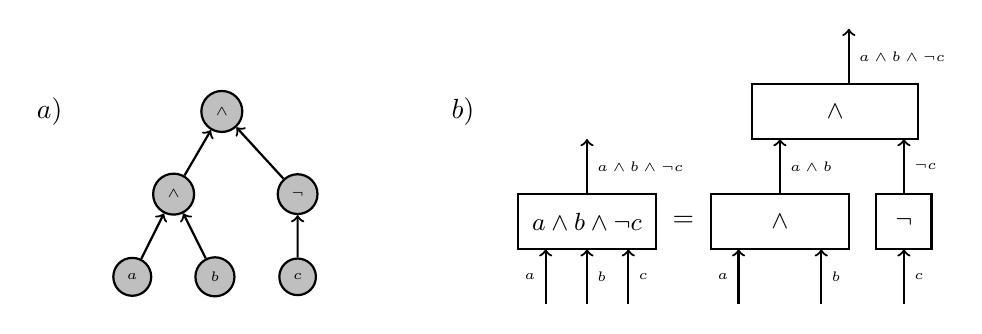
\begin{tikzpicture}[scale=0.35, yscale=-1, thick] % , baseline = -3.5pt

\begin{scope}[shift={(-15,0)}]

\node[anchor=center] (text) at (-3,-6) {${a)}$};

	\node [circle, draw, thick, fill=gray!50] (T1) at (0,0) {\tiny $\catvariableof{a}$};
	\node [circle, draw, thick, fill=gray!50] (T2) at (3,0) {\tiny $\catvariableof{b}$};
	\node [circle, draw, thick, fill=gray!50] (T3) at (6,0) {\tiny $\catvariableof{c}$};
	
	\node [circle, draw, thick, fill=gray!50] (and) at (1.5,-3) {\tiny $\land$};
	\node [circle, draw, thick, fill=gray!50] (not) at (6,-3) {\tiny $\lnot$};	
	
	\draw [->] (T1) -- (and);
	\draw [->] (T2) -- (and);
	
	\draw [->] (T3) -- (not);	
	
	\node [circle, draw, thick, fill=gray!50] (head) at (3.25,-6) {\tiny $\land$};
	
	\draw [->] (and) -- (head);
	\draw [->] (not) -- (head);			
\end{scope}

\node[anchor=center] (text) at (-3,-6) {${b)}$};

\draw[->] (0,1)--(0,-1) node[midway,left] {\tiny $\catvariableof{a}$}; 
\draw[->] (1.5,1)--(1.5,-1) node[midway,right] {\tiny $\catvariableof{b}$}; 
\draw[->] (3,1)--(3,-1) node[midway,right] {\tiny $\catvariableof{c}$}; 
\draw (-1,-1) rectangle (4, -3);
\node[anchor=center] (text) at (1.5,-2) {\small $\rencodingof{a \land b \land \lnot c}$};
\draw[->] (1.5,-3)--(1.5,-5) node[midway,right] {\tiny $\headvariableof{a \land b \land \lnot c}$}; 

\node[anchor=center] (text) at (5,-2) {${=}$};


\begin{scope}[shift={(7,0)}]

\draw[->] (0,1)--(0,-1) node[midway,left] {\tiny $\catvariableof{a}$}; 
\draw[->] (3,1)--(3,-1) node[midway,right] {\tiny $\catvariableof{b}$}; 
\draw[->] (6,1)--(6,-1) node[midway,right] {\tiny $\catvariableof{c}$}; 
	
\draw (-1,-1) rectangle (4, -3);
\node[anchor=center] (text) at (1.5,-2) {\small $\rencodingof{\land}$};

\draw[->] (1.5,-3) --(1.5,-5) node[midway,right]{\tiny $\headvariableof{a \land b}$};

\draw (5,-1) rectangle (7, -3);
\node[anchor=center] (text) at (6,-2) {\small $\rencodingof{\lnot}$};

\draw[->] (6,-3) --(6,-5) node[midway,right]{\tiny $\headvariableof{\lnot c}$};
	
\draw (0.5,-5) rectangle (6.5,-7);
\node[anchor=center] (text) at (3.5,-6) {\small $\rencodingof{\land}$};
	
\draw[->] (4,-7) -- (4,-9) node[midway,right] {\tiny $\headvariableof{a \land b \land \lnot c}$};

%\draw (3,-9) rectangle (5,-11);
%\node[anchor=center] (text) at (4,-10) {$\truevectorat{}$};

\end{scope}

\end{tikzpicture}
\end{center}
\caption{Decomposition of the formula tensor to $\exformula = a \land b \land \lnot c$ into unary (matrix) and binary (third order tensor) cores.
	a) Visualization of $\exformula$ as a graph. %(\red{Exploiting the duality between tensor networks on hypergraphs and graphical models \cite{robeva_duality_2019} })
	b) Dual Tensor Network decomposition of $\exformula$.
	We can make use of the invariance of a Hadamard product with a constant tensor $\ones$ and thus not draw axis to atoms not affected by a formula.}
\label{fig:FTDecomposition}
\end{figure}





\begin{remark}[$\htformat$ Interpretation of Formula Tensor Networks]\label{rem:HTDecomFT}
	The sketched decomposition of the formula tensor into a network is a hierarchical tree decomposition of the formula tensor, which we will describe in more detail in Section~\ref{sec:HT}.
	At each decomposition of a formula into subformulas, two subspaces spanned by the respective atomic spaces are selected. 
\end{remark}


\subsubsection{Syntactical decomposition of formulas}\label{sec:termClauseDecomposition}

% Decomposition in case of missing 
We have seen how the decomposition of complex formulas into connectives acting on the component formulas can be exploited to find effective representations of the semantics by tensor networks.
Here the question arises here, how to perform such decompositions in case of a missing syntactical representation of a formula.
By Definition~\ref{def:formulas} any binary tensor is a formula.
We show in the following, how we can find a syntactic specification of a formula given its tensor.

%
%Let us now show that any formula tensor can be decomposed into a network of these connective symbols and atomic formula tensors.


\begin{definition}[Terms and Clauses]\label{def:clauses}
	Given two disjoint subsets $\nodes_0$ and $\nodes_1$ of the $[\atomorder]$, the corresponding term is the formula defined on the indices $\catindices\in\atomstates$ by
		\[ \termof{\nodes_0}{\nodes_1}
		=\left( \bigwedge_{\atomenumerator\in\nodes_0} \lnot\formulaof{\atomenumerator} \right)  \land \left( \bigwedge_{\atomenumerator\in\nodes_1} \formulaof{\atomenumerator} \right)  \]
	and the corresponding clause is the formula defined on the indices $\catindices\in\atomstates$ by
		\[ \clauseof{\nodes_0}{\nodes_1}
		=\left( \bigvee_{\atomenumerator\in\nodes_0} \formulaof{\atomenumerator} \right)  \lor \left( \bigvee_{\atomenumerator\in\nodes_1} \lnot\formulaof{\atomenumerator} \right)  \, , \]
	where by $\land_{\atomenumerator\in\nodes}$ and $\lor_{\atomenumerator\in\nodes}$ we refer to the $n$-ary connectives $\land$ and $\lor$.
	%We call the clause a minterm, if $\nodes_0\cup\nodes_1 = [\atomorder]$.
	We call the term a minterm and the clause a maxterm, if $\nodes_0\cup\nodes_1 = [\atomorder]$.
\end{definition}

%% 
Terms and Clauses have for any index tuple $\catindexof{[\atomorder]}$ a polynomial representation by
		\[ \termof{\nodes_0}{\nodes_1}[\shortcatvariables=\catindexof{[\atomorder]}] 
		= \left( \prod_{\atomenumerator \in \nodes_0} (1-\catindexof{\atomenumerator}) \right)
		\left(  \prod_{\atomenumerator \in \nodes_1} \catindexof{\atomenumerator} \right) \]
and
		\[ \clauseof{\nodes_0}{\nodes_1}[\shortcatvariables=\catindexof{[\atomorder]}] 
		= 1 - \left( \prod_{\atomenumerator \in \nodes_0} (1-\catindexof{\atomenumerator})\right)
		\left(  \prod_{\atomenumerator \in \nodes_1} \catindexof{\atomenumerator} \right) \, . \]


\begin{lemma}\label{lem:termClauseOneHot}
	Terms are contractions of one-hot encodings, that is for any disjoint subsets $\nodes_0,\nodes_1\subset[\atomorder]$ we have
		\[ \termof{\nodes_0}{\nodes_1}[\shortcatvariables] = \contractionof{\onehotmapof{\{\atomlegindexof{k}=0 : k \in \nodes_0 \} \cup \{\atomlegindexof{k}=1 : k \in \nodes_1\}}}{\shortcatvariables} \, . \]
	Clauses are substractions of one-hot encodings from the trivial tensor, that is for any disjoint subsets $\nodes_0,\nodes_1\subset[\atomorder]$ we have
		\[ \clauseof{\nodes_0}{\nodes_1}[\shortcatvariables] = 
		\onesat{\shortcatvariables} -
		\contractionof{\onehotmapof{\{\atomlegindexof{k}=0 : k \in \nodes_0 \} \cup \{\atomlegindexof{k}=1 : k \in \nodes_1\}}}{\shortcatvariables} \, . \]
\end{lemma}


	
%
The reference of the formulas in the case $\nodes_0\dot{\cup}\nodes_1 = [\atomorder]$ as minterms and maxterms is due to the fact, that minterms are formulas with unique models and maxterms are formulas with a unique world not satisfying the formula.
% Enumeration by $\atomstates$
We use this insight and enumerate maxterms and minterms by the index $\catindex\in\atomstates$ of the unique world where the minterm is satisfied, respectively the maxterm is not satisfied.
For any $\nodes_0\dot{\cup}\nodes_1 = [\atomorder]$ we take the index tuple $\catindices$ where $\catindexof{\atomenumerator}=0$ if $\atomenumerator\in\nodes_0$ and $\catindexof{\atomenumerator}=1$ if $\atomenumerator\in\nodes_1$ and define
\begin{align*}
	\maxtermof{\catindices} = \clauseof{\nodes_0}{\nodes_1} \quad \text{and} \quad \mintermof{\catindices} = \termof{\nodes_0}{\nodes_1} \, .
\end{align*}


\begin{corollary}
	Minterms are basis elements of the tensor space, that is for any $\catindices\in\atomstates$ we have
	\begin{align*}
		\mintermof{\catindices} = \onehotmapof{\catindices}
	\end{align*}
	Maxterms are substraction of basis elements from the trivial tensor, that is for any $\catindices\in\atomstates$ we have
	\begin{align*}
		\maxtermof{\catindices} = \onesat{\shortcatvariables} - \onehotmapof{\catindices} \, .
	\end{align*}
\end{corollary}
\begin{proof}
	Follows from Lemma~\ref{lem:termClauseOneHot}, since when $\nodes_0\cup\nodes_1 = [\atomorder]$ the contractions of the one-hot encodings coincides with the one-hot encoding of a fully specified state.
\end{proof}


Based on this insight, we can decompose any propositional formula into a conjunction of maxterms or a disjunction of minterms as we show next.

\begin{theorem}\label{the:tensorToMaxMinTerms}
	For any binary tensor $\hypercoreat{\shortcatvariables}\in\bigotimes_{\atomenumeratorin}\rr^2$ with two-dimensional axes we have
	\begin{align*}
		\hypercoreat{\shortcatvariables} = \left( \bigvee_{\catindices : \hypercoreat{\shortcatvariables=\catindexof{[\atomorder]}}=1} 
		\termof{
		\{\atomenumerator : \catindexof{\atomenumerator}=0\}
		}{
		\{\atomenumerator: \catindexof{\atomenumerator}=1\}
		} 
		\right)
		[\shortcatvariables] 
	\end{align*}
	and
	\begin{align*}
		\hypercoreat{\shortcatvariables} = \left( \bigwedge_{\catindices : \hypercoreat{\shortcatvariables=\catindexof{[\atomorder]}}=0} 
		\clauseof{
		\{\atomenumerator : \catindexof{\atomenumerator}=0\}
		}{
		\{\atomenumerator: \catindexof{\atomenumerator}=1\}
		} 
		\right)
		[\shortcatvariables] \, .
	\end{align*}
\end{theorem}
\begin{proof}
	To show the representation by minterms we use the decomposition
	\begin{align*}
		\hypercoreat{\shortcatvariables}  = \sum_{\catindexof{[\atomorder]} : \hypercoreat{\catvariableof{[\atomorder]}=\catindexof{[\atomorder]}} = 1} \onehotmapofat{\catindexof{[\atomorder]}}{\shortcatvariables}
	\end{align*}
	and notice that each term in the disjunction modifies the formula by adding respective world $\catindexof{[\atomorder]}$ to the models of the formula.
	To show the representation by maxterms we use the decomposition
	\begin{align*}
		\hypercoreat{\shortcatvariables}  = \onesat{\shortcatvariables} \quad - \sum_{\catindexof{[\atomorder]} : \hypercoreat{\catvariableof{[\atomorder]}=\catindexof{[\atomorder]}} = 0} \onehotmapofat{\catindexof{[\atomorder]}}{\shortcatvariables}
	\end{align*}
	and notice that each term in the conjunction modifies the formula by removing the respective world $\catindexof{[\atomorder]}$ from the models of the formula.	
	Thus, both decompositions are propositional formulas with the same set of models as the formula $\hypercore$ and are thus identical to $\hypercore$.
\end{proof}


% Canonical normal forms
The decompositions found in Theorem~\ref{the:tensorToMaxMinTerms} are also called canonical normal forms to propositional formulas $\hypercoreat{\shortcatvariables}$.

%\begin{theorem}\label{the:FormulaToTensor}
%	For any binary tensor $\hypercore\in\bigotimes_{\atomenumeratorin}\rr^2$ with two-dimensional axes we find a formula $\exformula$ in propositional syntax such that
%		\[ \hypercore = \exformula \, . \]
%\end{theorem}
%\begin{proof}
%	For any such $\hypercore$ we construct the formula
%		\[ \exformula^{\hypercore} = \lor_{\atomindices : \hypercore_{\atomindices}=1} \clauseof{\{\atomenumerator : \atomlegindexof{\atomenumerator=0}\}}{\{\atomenumerator : \atomlegindexof{\atomenumerator=1}\}}  \, . \]
%	Since the clauses are basis vectors and $\hypercore$ is binary we get
%		\[ \exformula^{\hypercore} = \sum_{\atomindices : \hypercore_{\atomindices}=1} \onehotmapof{\atomindices} = \hypercore \, .   \] 
%%	Take for any $\ftensor$ the formula
%%		\[ \exformula = \lor_{\atomindices : \ftensor_{:,\atomindices} = \tbasis}
%%		 \left( \land_{\atomenumerator : \atomlegindexof{\atomenumerator} =1} \atomicformulaof{\atomenumerator}\right)
%%		\left( \land_{\atomenumerator : \atomlegindexof{\atomenumerator} =0} \lnot \atomicformulaof{\atomenumerator} \right) \]
%%	to show the claim.
%\end{proof}

%
%In the proof of Theorem~\ref{the:FormulaToTensor} we only applied the connectives $\land,\lor$ and $\lnot$ in the construction of syntactical specifications of formulas. 
%These connectives thus universal in the sense, that their combinations are representing any binary tensor as in Theorem~\ref{the:FormulaToTensor}.
%This observation can be connected with the theory of normal forms, where arbitrary formulas can be syntactically represented by these connectives only (often called logical equivalent, which in our case means identical formula tensor). 




%% Universality of representations
\begin{remark}[Efficient Representation in Propositional Syntax]
	% Relation with binary CP
	The decomposition in Theorem~\ref{the:tensorToMaxMinTerms} is a basis CP decomposition of the binary tensor and will further be investigated in Chapter~\ref{cha:sparseTC}. 
	The formulas constructed in the proof of Theorem~\ref{the:tensorToMaxMinTerms} are however just one possibility to represent a formula tensor in propositional syntax.
	Typically there are much sparser representations for many formula tensors, in the sense that less connectives and atomic symbols are required.
	Having such a sparser syntactical description of a propositional formula can be exploited to find a shorter conjunctive normal form of the formula and construct a sparse polynomial based on similar ideas as in Theorem~\ref{the:tensorToMaxMinTerms}.
	%One way to eliminate syntactical redundancies are through schemes for decompositions called normal forms, for example the Conjunctive Normal Form (CNF) or the Disjunctive Normal Form (DNF).
	We will provide such constructions in Chapter~\ref{cha:sparseTC}, where we show that dropping the demand of directionality and investigating binary CP Decompositions will improve the sparsity of the polynomial formula representation.
\end{remark}


\subsection{Discussion and Outlook}

Further study of representing Knowledge Bases based on Tensor Networks of its formulas in Section~\ref{sec:hardNetworks} (see Theorem~\ref{the:conDecKB}).




%\subsection{Knowledge Bases as Tensor Networks}
%
%%We here aim at a representation of the semantics of a Knowledge Base, whereas traditional systems store the Knowledge Base exploiting the syntax (i.e.storing the known formulas in the propositional syntax).
%% In this formalism a Knowledge Base is represented by its models, i.e. worlds where it is true.
%
%% Representation of multiple formuals
%Let us investigate how we to store a Knowledge Base of formulas $\exformula\in\formulaset$
%\begin{align}
%	\kb = \land_{\exformulain}\exformula \, .
%\end{align}
%
%One obvious way is to use the scheme of Theorem~\ref{the:compositionByContraction} and contract the relational encoded formulas with a conjunction encoding, that is
%\begin{align}
%	\rencodingofat{\kb}{\shortcatvariables,\catvariableof{\kb}}
%	= \contractionof{
%	\{\rencodingofat{\land}{\catvariableof{\formulaset}, \catvariableof{\kb}}\}
%	\cup\{\rencodingofat{\exformula}{\shortcatvariables,\catvariableof{\exformula}}  : \exformula \in \formulaset \}}{\shortcatvariables,\catvariableof{\kb}}
%\end{align}
%Here we denote by $\land$ the $\cardof{\formulaset}$-ary conjunction, which is well-defined by Remark~\ref{rem:naryConnectives}.
%
%% Simpler by effective calculus
%It is however possible to execute the $\cardof{\formulaset}$-ary conjunction by effective calculus (see Section~\ref{sec:effectiveGroundingCalculus}) and we have
%\begin{align}
%	\kb[\shortcatvariables]= \contractionof{\{\formulaat{\shortcatvariables} : \exformulain \}}{\shortcatvariables} \, .
%\end{align}










